\documentclass[10pt,twocolumn,letterpaper]{article}

\usepackage{iccv}
\usepackage{times}
\usepackage{epsfig}
\usepackage{graphicx}
\usepackage{amsmath}
\usepackage{amssymb}
\usepackage{mathrsfs}
\DeclareMathOperator{\E}{\mathbb{E}}

% Include other packages here, before hyperref.

% If you comment hyperref and then uncomment it, you should delete
% egpaper.aux before re-running latex.  (Or just hit 'q' on the first latex
% run, let it finish, and you should be clear).
\usepackage[pagebackref=true,breaklinks=true,letterpaper=true,colorlinks,bookmarks=false]{hyperref}

\iccvfinalcopy % *** Uncomment this line for the final submission

\def\iccvPaperID{2685} % *** Enter the ICCV Paper ID here
\def\httilde{\mbox{\tt\raisebox{-.5ex}{\symbol{126}}}}

% Pages are numbered in submission mode, and unnumbered in camera-ready
\ificcvfinal\pagestyle{empty}\fi
\begin{document}

%%%%%%%%% TITLE
%\title{Realistic Video Face Retargeting Using Conditional Generative Adversarial Networks}
% \title{Animating Realistic Dynamic Facial Textures from a Single Image using GANs}
\title{Realistic Dynamic Facial Textures from a Single Image using GANs - Supplementary Material}
%\title{Animating Realistic Dynamic Facial Textures using Generative Adversarial Networks}

%% \author{First Author\\
%% Institution1\\
%% Institution1 address\\
%% {\tt\small firstauthor@i1.org}
%% % For a paper whose authors are all at the same institution,
%% % omit the following lines up until the closing ``}''.
%% % Additional authors and addresses can be added with ``\and'',
%% % just like the second author.
%% % To save space, use either the email address or home page, not both
%% \and
%% Second Author\\
%% Institution2\\
%% First line of institution2 address\\
%% {\tt\small secondauthor@i2.org}
%% }

\maketitle
%\thispagestyle{empty}

\section{Additional Results and Evaluations}

% The video

More results and evaluations on video sequences of various test subjects can be seen in the supplemental video included with this submission. We show examples of the facial albedo textures that are inferred given the target identity and source expression sequence (with the estimated environmental lighting factored out to allow for relighting the textured faces under different illumination conditions).

The retargeting and compositing results seen in the video demonstrate that, in addition to synthesizing the mouth interior, our system is able to generate subtle wrinkles and deformations in the face texture that are too small to be represented in the mesh used for fitting the face model to the subject, but do indeed enhance the realism of the synthesized sequence of expressions generated for the target image. (We show these sequences slowed down to allow for better visualization of the transient details created for each expression.) Furthermore, we note that the wrinkles generated by this system do not correspond directly to those of the source expressions in the video, but rather vary depending on factors such as the appearance and age of the person depicted in the target image (see, for example, the retargeting to images of Brad Pitt and Angelina Jolie in the section ``Retargeting Results and Comparison with Static Texture'' in the supplemental video).

Our approach to compositing the final rendered image of the target subject into the source sequence requires that the faces be front-facing. However, we note that our network architecture can synthesize dynamic textures even for non-frontal viewpoints of the source subject, as seen in Fig.~\ref{fig:replaceres}. Cases showing a frontal source subject animating a non-frontal target subject can be seen in Fig.~\ref{fig:replaceres2}, although we note that in this case there are artifacts in the occluded regions that may be visible in the final animation. Additional retargeting and compositing results can be found in Fig.~\ref{fig:compositenew}.

%% \paragraph{}

\section{Implementation, Training and Performance Details}

Our networks are implemented and trained using the Torch7 framework, using an NVIDIA Titan GPU to accelerate the training and inference. Fig.~\ref{fig:error} shows the loss on the training and validation dataset for both the generative and discriminative networks.

Below we list the average per-frame execution time for each stage in our texture generation and compositing pipeline.

While our implementation of the 3D face model fitting approach described in Section 4 is implemented on the CPU and does not run in realtime, we note that [Thies et al. 2016] demonstrate that such an approach can be implemented in parallel on the GPU to achieve realtime performance. Furthermore, the mouth interior synthesis approach described in Section 5.4 of the paper is implemented in Matlab using a single thread for processing, and thus could be further optimized using parallel processing. Thus, while the approach used for replacing the faces in the source video sequence with the rendered target faces is not designed to run in realtime, it should be possible to further optimize the other stages of the pipeline to run at interactive framerates.

%  While the approach used for compositing the .

% albedo, relight
% wrinkles not rep. in mesh expressions
% upsampled
% realtime f2f, cpu
% parallelized, optimized

% \vfill\eject

\begin{enumerate}
\item 3D face model fitting (Section 4): 5.6 seconds
\item Texture inference (Section 5): 12 milliseconds.
\item Mouth interior synthesis (Section 5.4): 156 milliseconds.
\item Video face replacement (Section 6): 4.5 seconds.
\end{enumerate}

%% \paragraph{}

%% \section{}

%% \paragraph{}

%% \input{implementation_details}
%% \input{additional_results}
%% \input{evaluations}
% TODO: reference to the table. The caption should be fleshed out.
\begin{figure}[th]
\begin{center}
  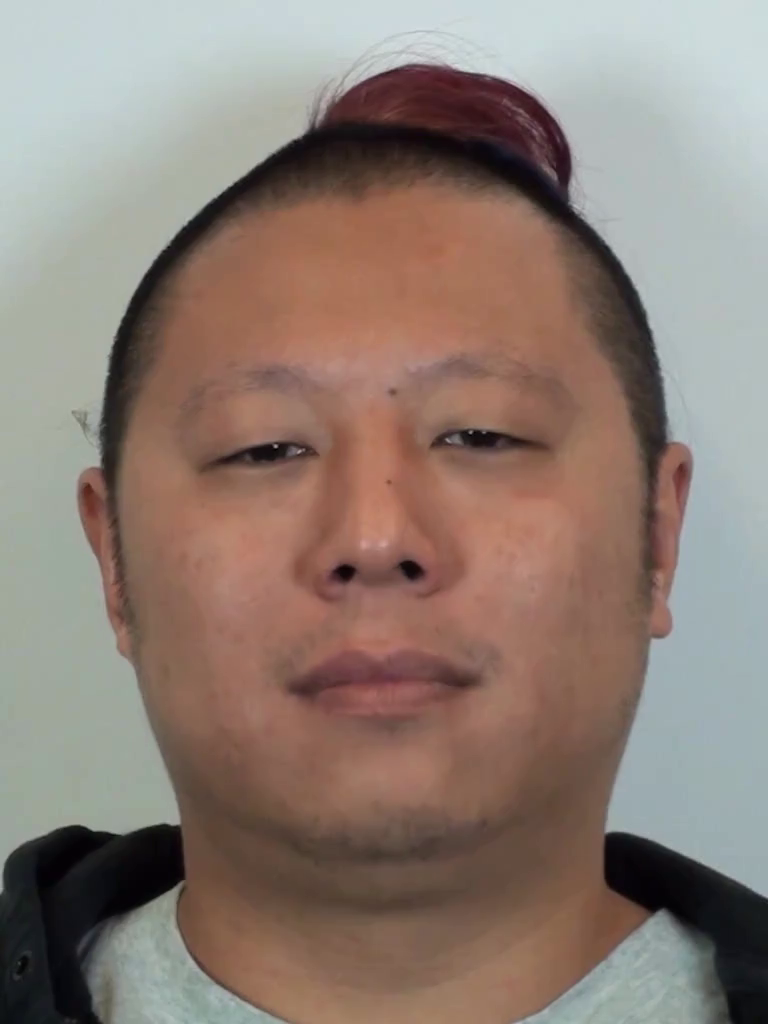
\includegraphics[width=0.32\columnwidth]{figures/kylehao_transfer/raw000001.png} \\
  
\includegraphics[width=0.32\columnwidth]{figures/kylehao_transfer/raw000762.png} 
  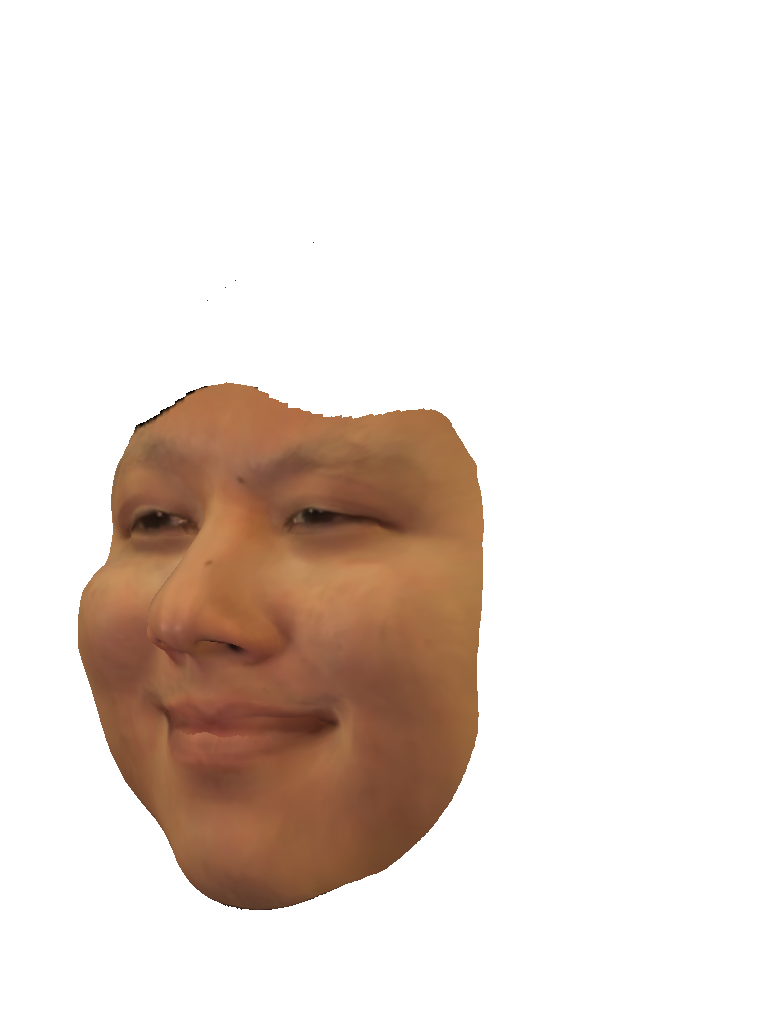
\includegraphics[width=0.32\columnwidth]{figures/kylehao_transfer/static_000762.png}
  
\includegraphics[width=0.32\columnwidth]{figures/kylehao_transfer/dynamic_000762.png} \\
  
\includegraphics[width=0.32\columnwidth]{figures/kylehao_transfer/raw000837.png}
  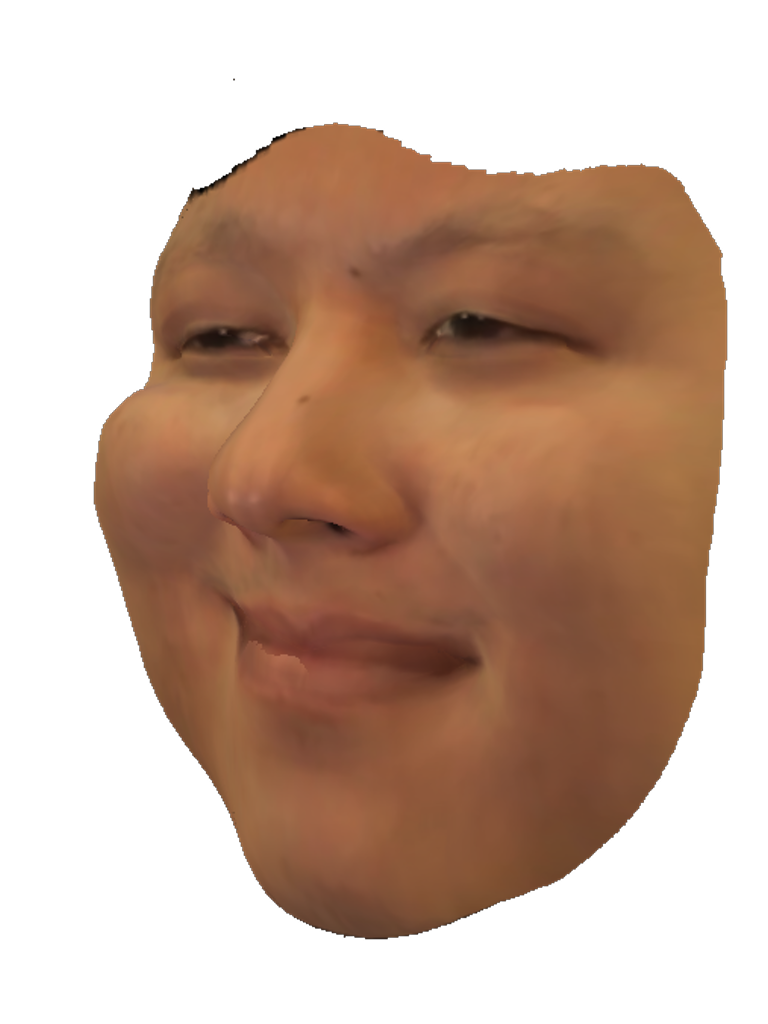
\includegraphics[width=0.32\columnwidth]{figures/kylehao_transfer/static_000837.png}
  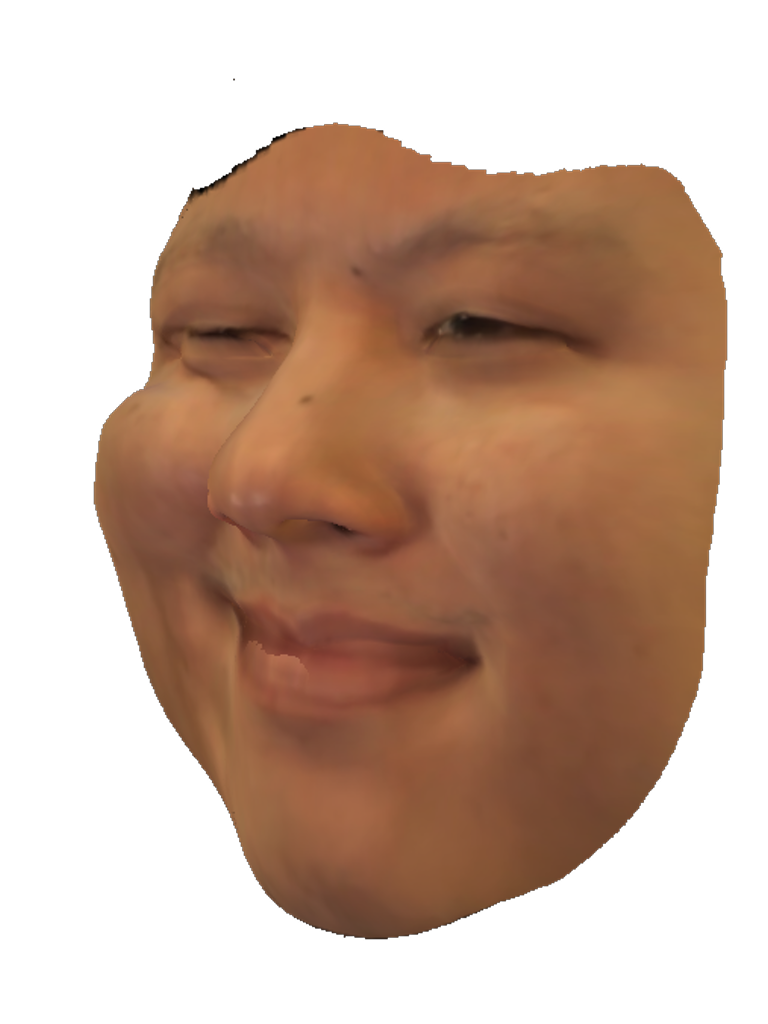
\includegraphics[width=0.32\columnwidth]{figures/kylehao_transfer/dynamic_000837.png} \\
  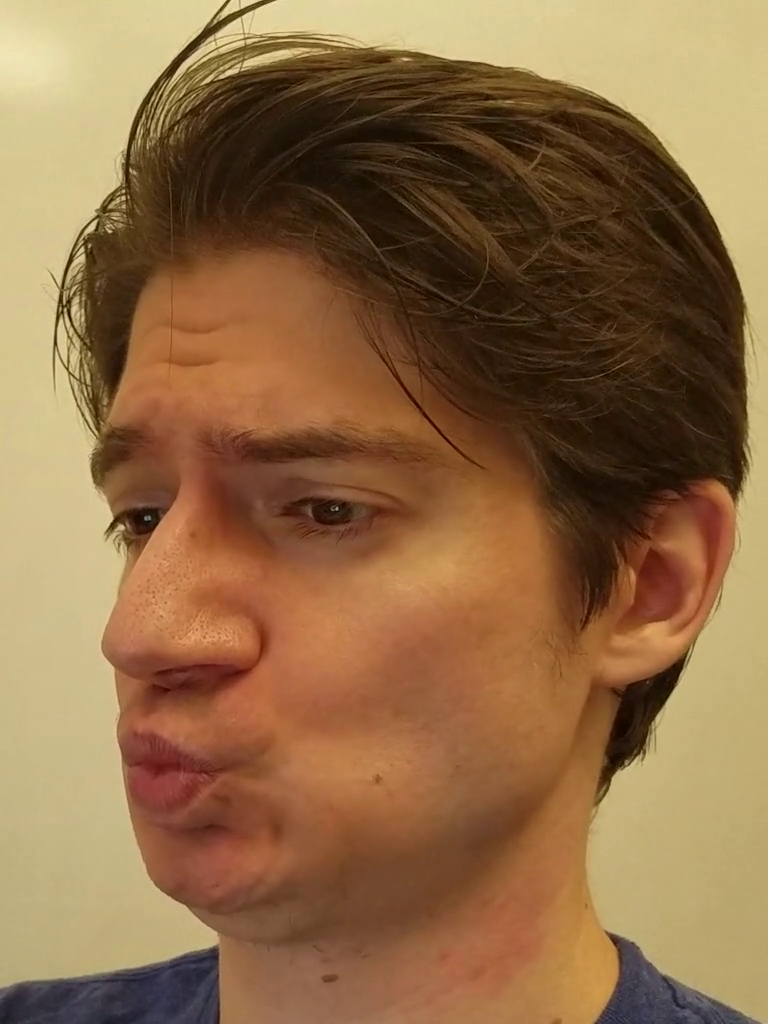
\includegraphics[width=0.32\columnwidth]{figures/kylehao_transfer/raw000455.png}
  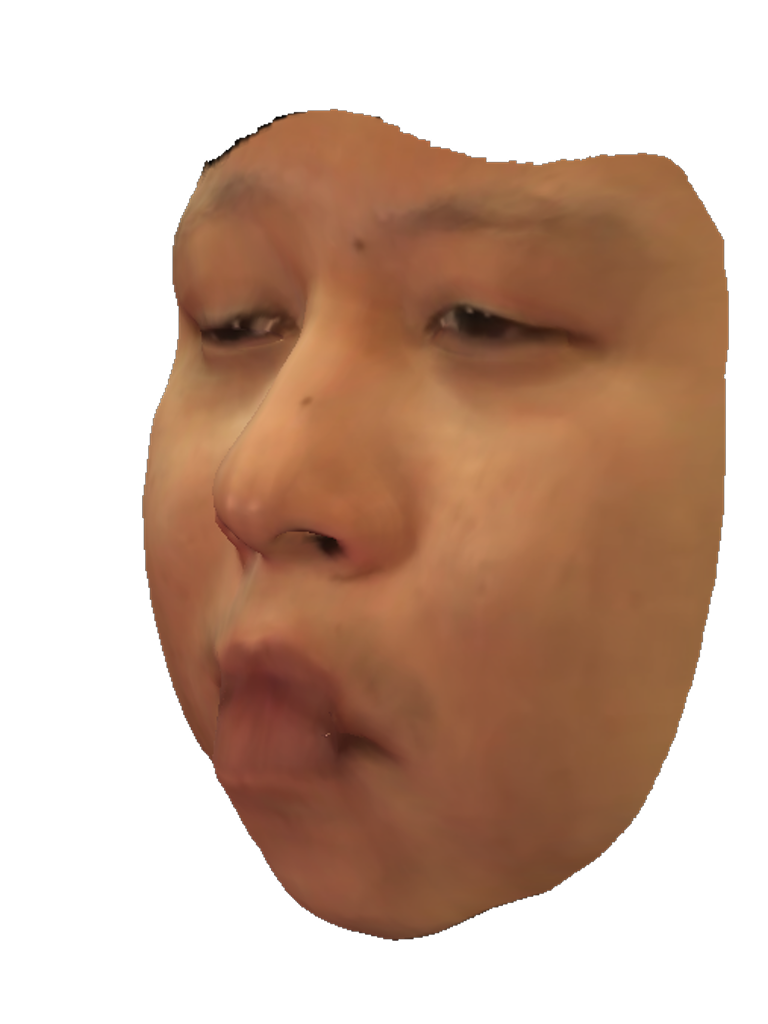
\includegraphics[width=0.32\columnwidth]{figures/kylehao_transfer/static_000455.png}
  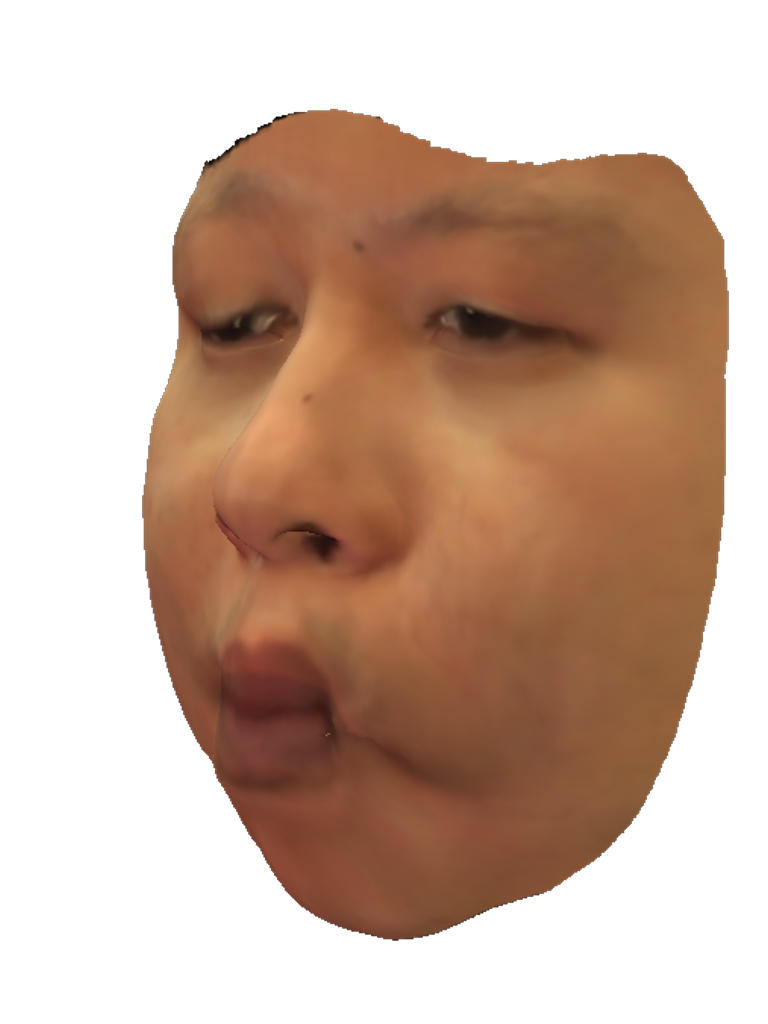
\includegraphics[width=0.32\columnwidth]{figures/kylehao_transfer/dynamic_000455.png} \\
  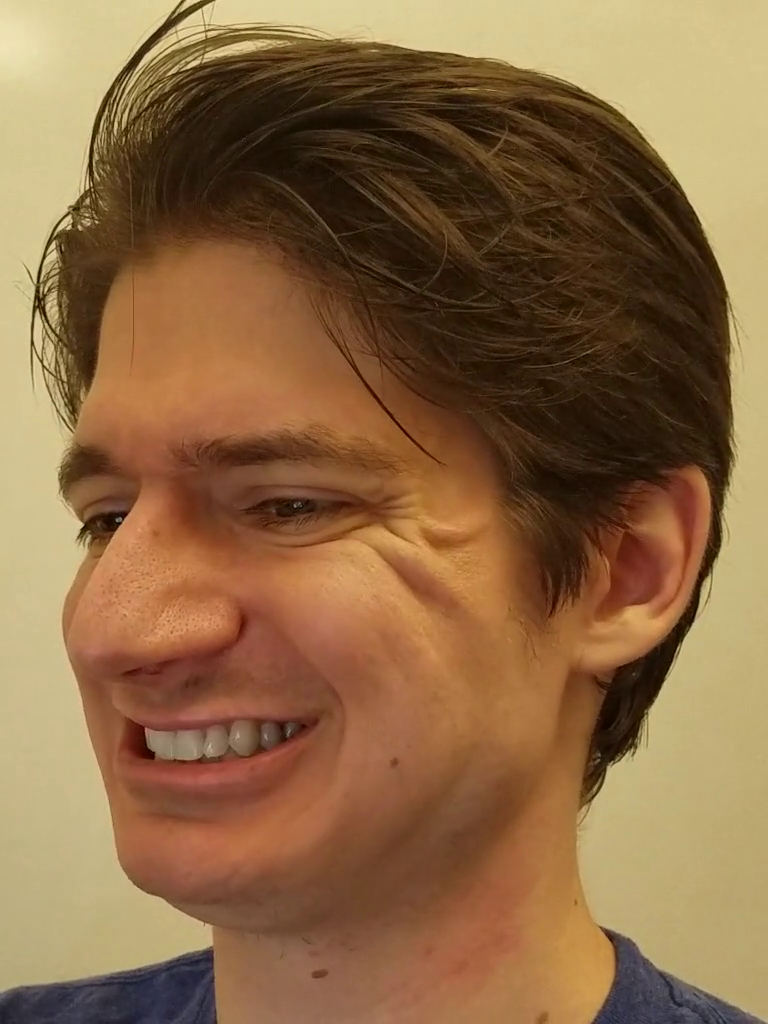
\includegraphics[width=0.32\columnwidth]{figures/kylehao_transfer/raw000066.png}
  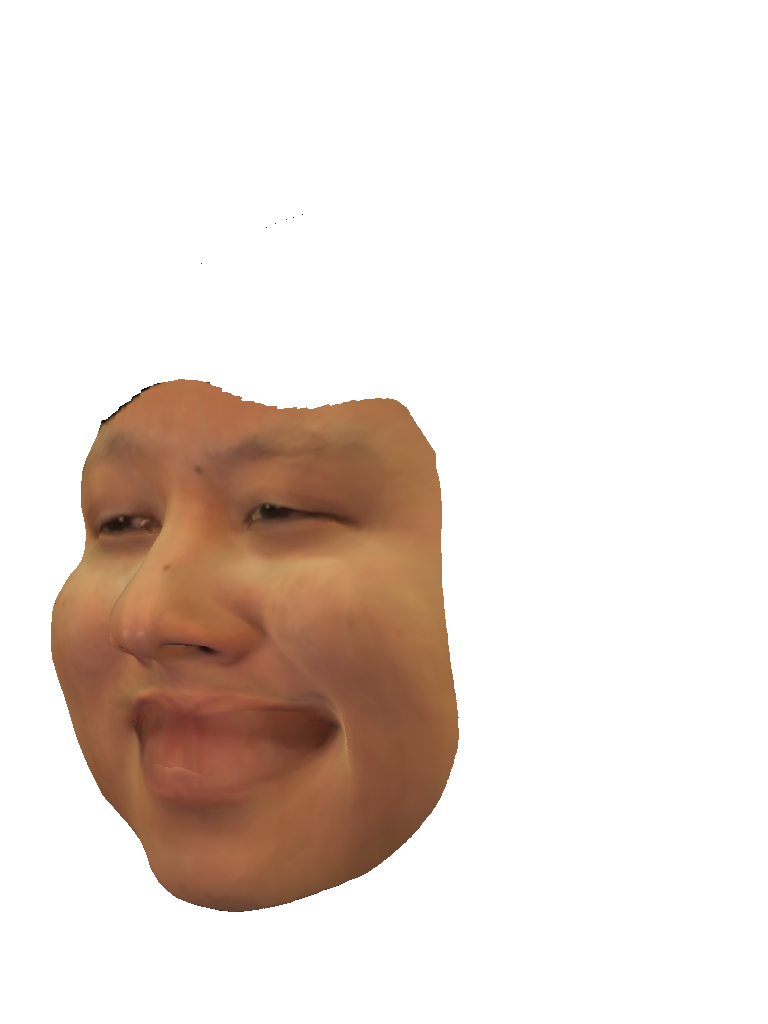
\includegraphics[width=0.32\columnwidth]{figures/kylehao_transfer/static_000066.png}
  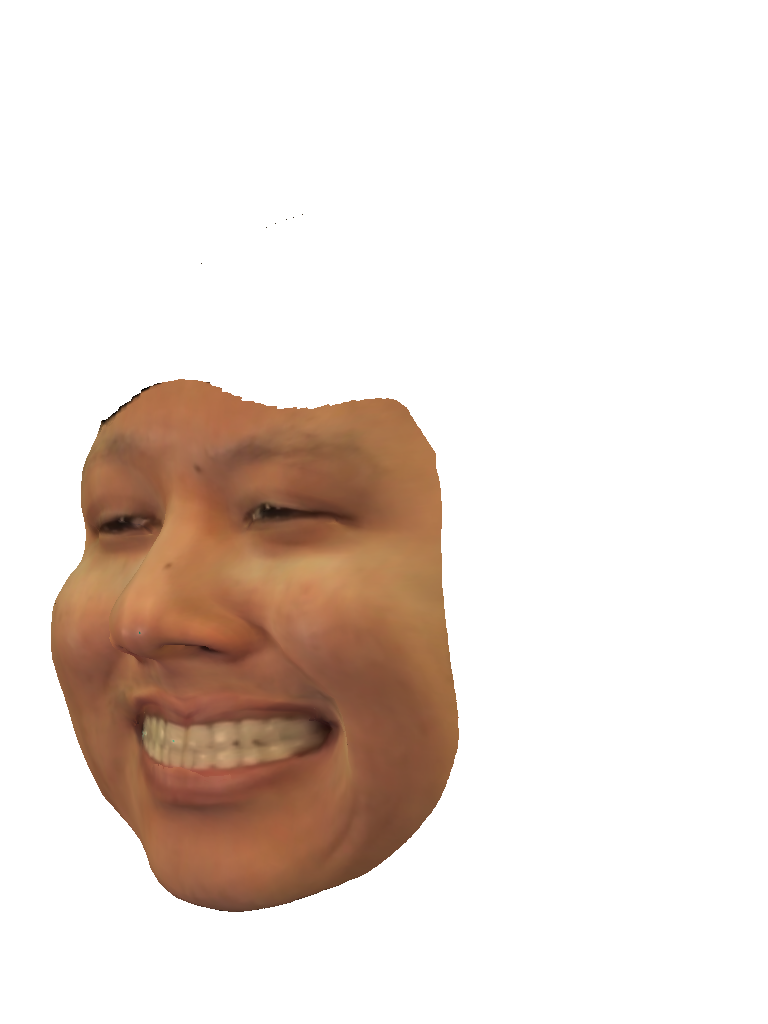
\includegraphics[width=0.32\columnwidth]{figures/kylehao_transfer/dynamic_000066.png}
\end{center}
   \caption{Non-frontal face reenactment. The top row displays the target image. In the remaining rows, from left to right: the source image, the rendered static texture and the rendered dynamic texture. We can see that the dynamic texture contains more subtle details such as wrinkles, resulting in a more expressive and plausible image of the target subject. Also note that the synthesized mouth interior results in much more plausible renderings when the mouth is open.}
   \vspace{-0.05in}
\label{fig:replaceres}
\end{figure}

\begin{figure}[th]
\begin{center}
  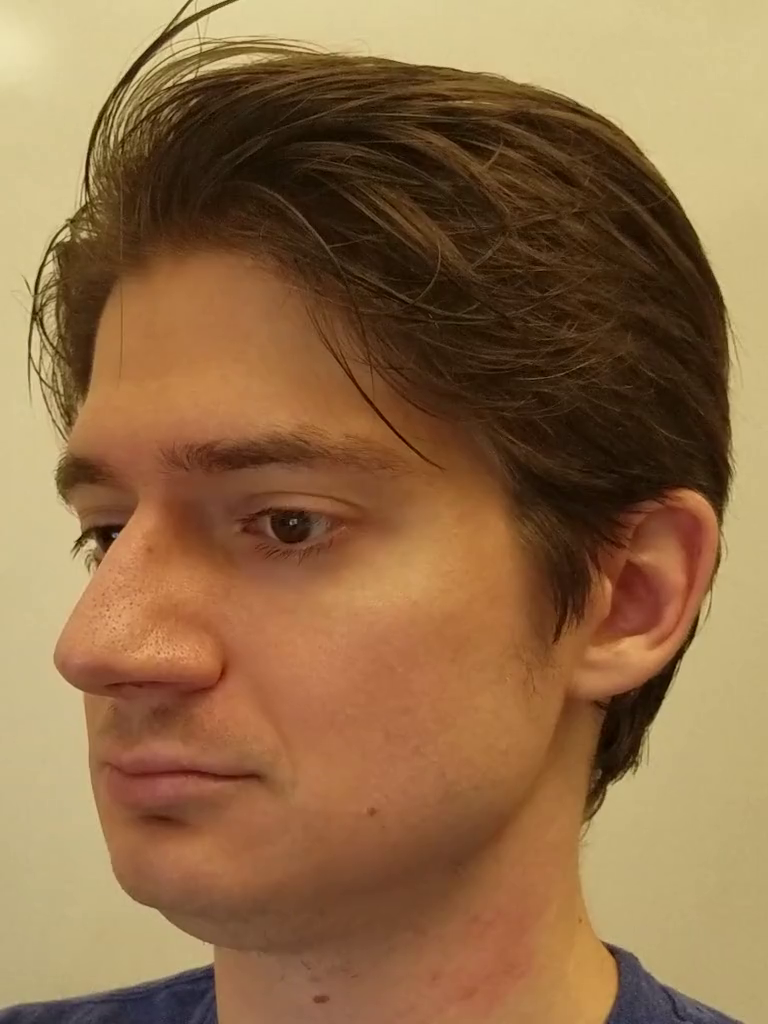
\includegraphics[width=0.32\columnwidth]{figures/haokyle_transfer/raw000001.png} \\
  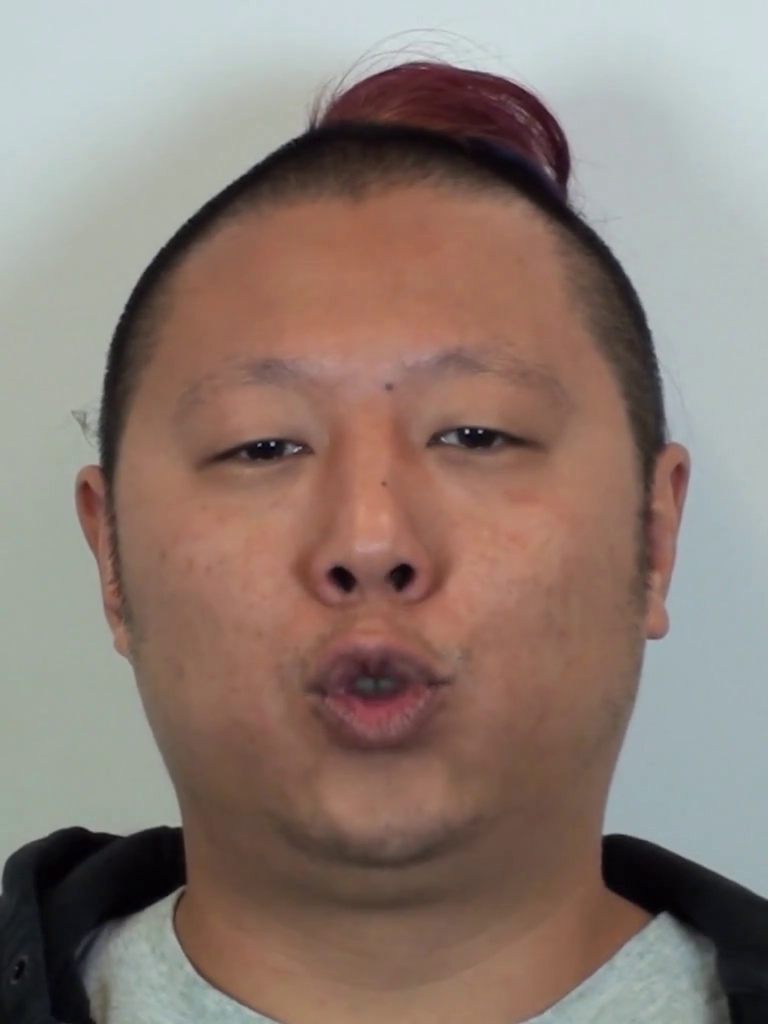
\includegraphics[width=0.32\columnwidth]{figures/haokyle_transfer/raw000165.png} 
  %% \includegraphics[width=0.32\columnwidth]{figures/haokyle_transfer/static_000165.png}
  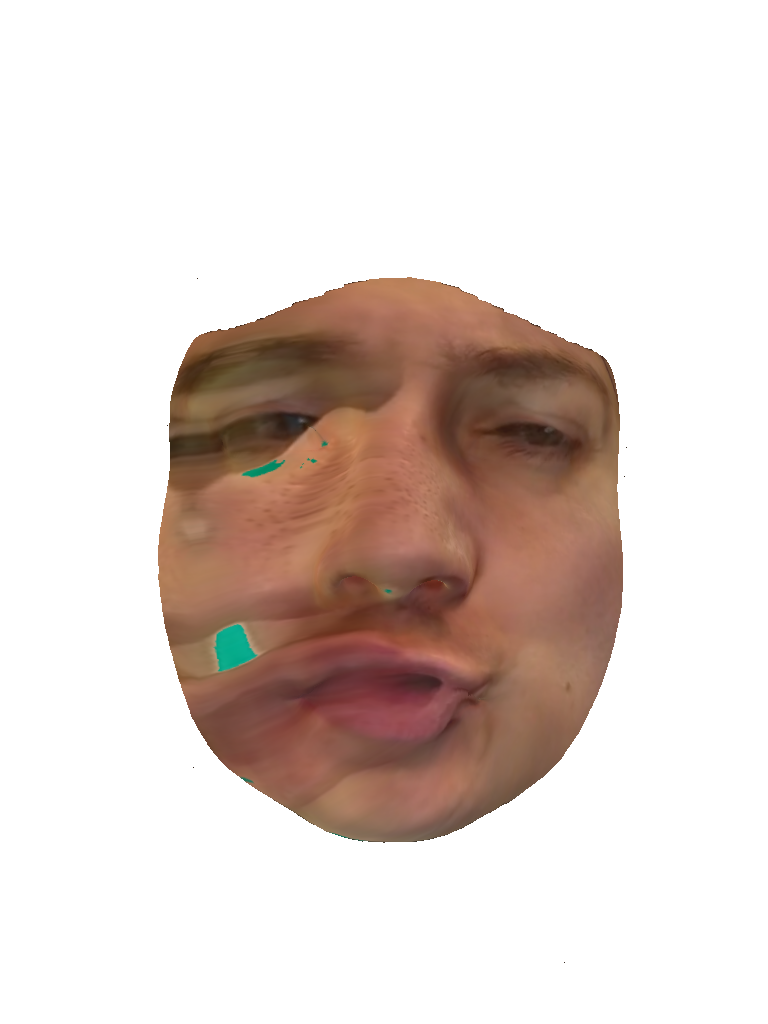
\includegraphics[width=0.32\columnwidth]{figures/haokyle_transfer/dynamic_000165.png} \\
  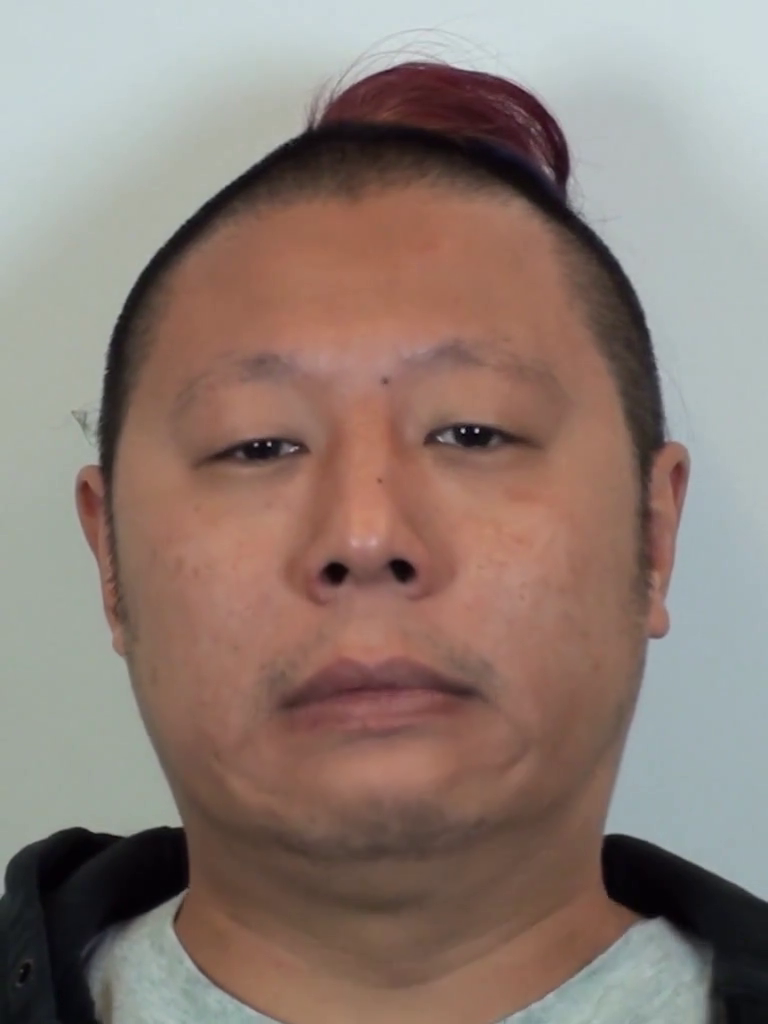
\includegraphics[width=0.32\columnwidth]{figures/haokyle_transfer/raw000103.png}
  %% \includegraphics[width=0.32\columnwidth]{figures/haokyle_transfer/static_000103.png}
  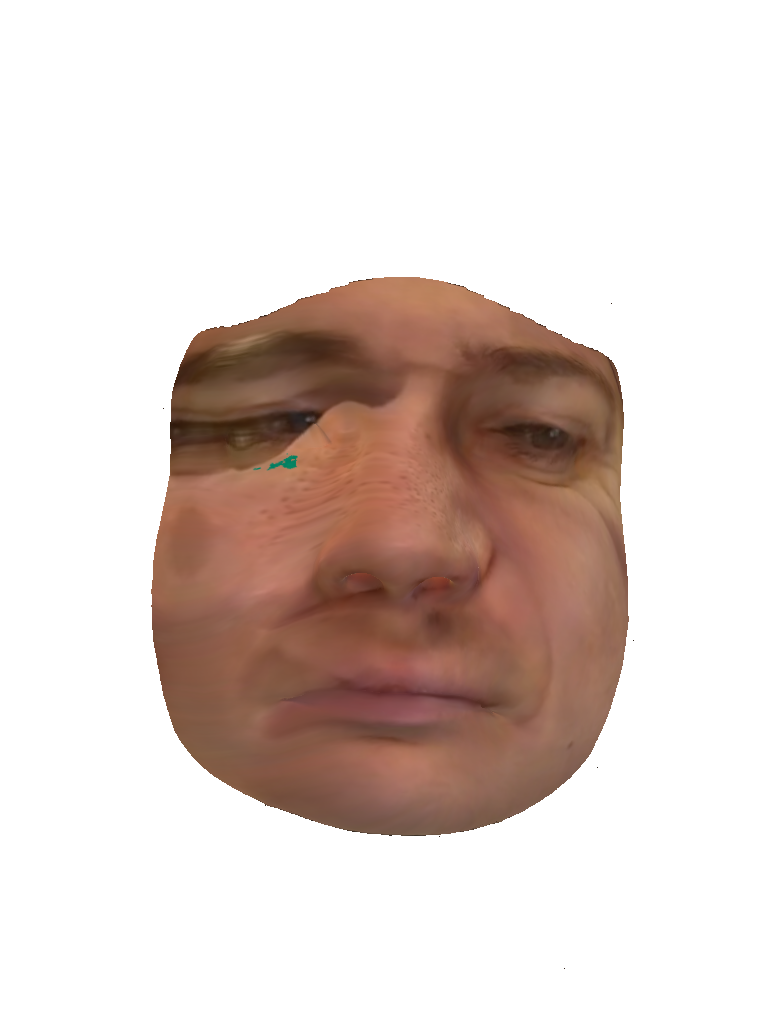
\includegraphics[width=0.32\columnwidth]{figures/haokyle_transfer/dynamic_000103.png} \\
  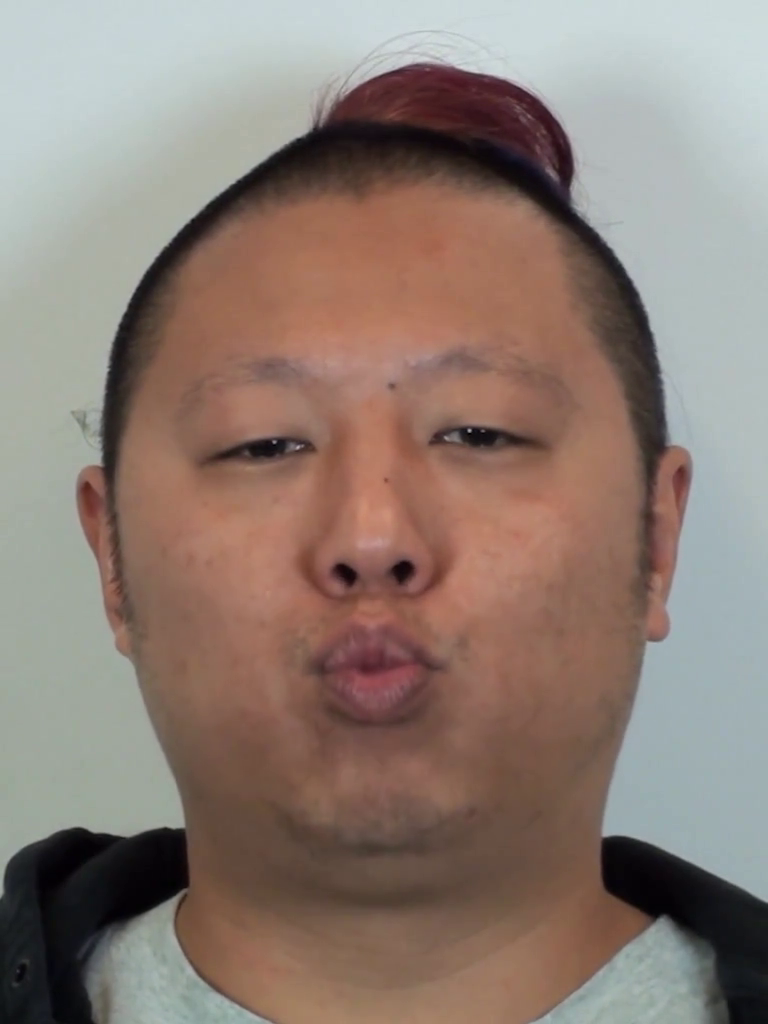
\includegraphics[width=0.32\columnwidth]{figures/haokyle_transfer/raw000356.png}
  %% \includegraphics[width=0.32\columnwidth]{figures/haokyle_transfer/static_000356.png}
  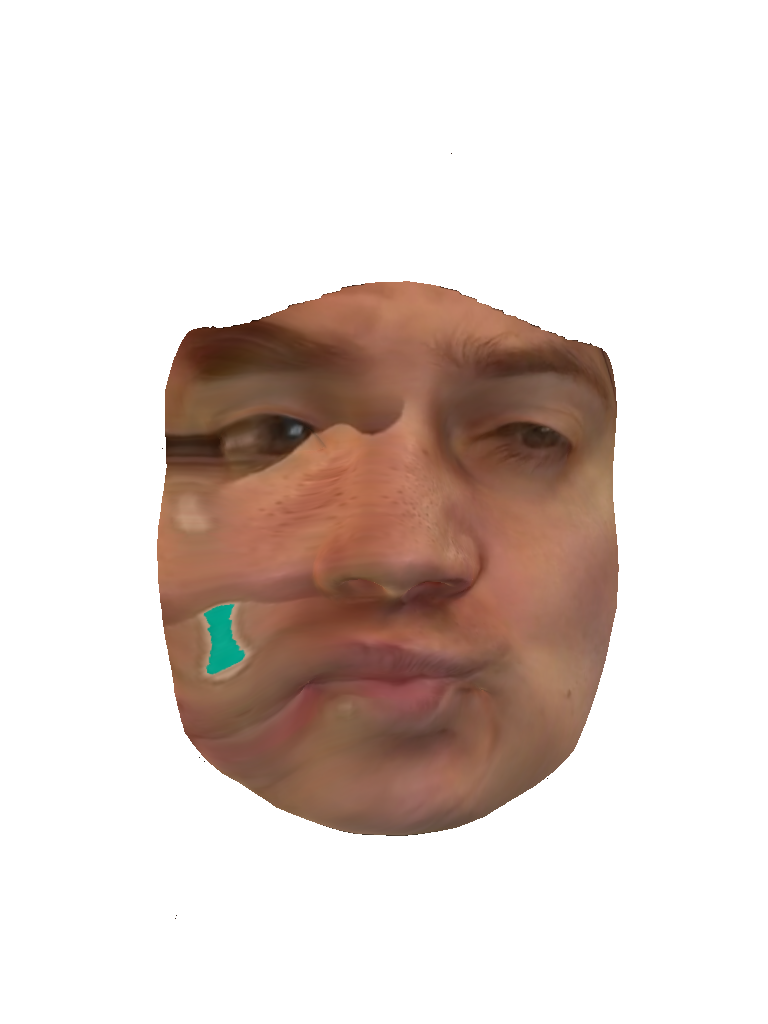
\includegraphics[width=0.32\columnwidth]{figures/haokyle_transfer/dynamic_000356.png} \\
  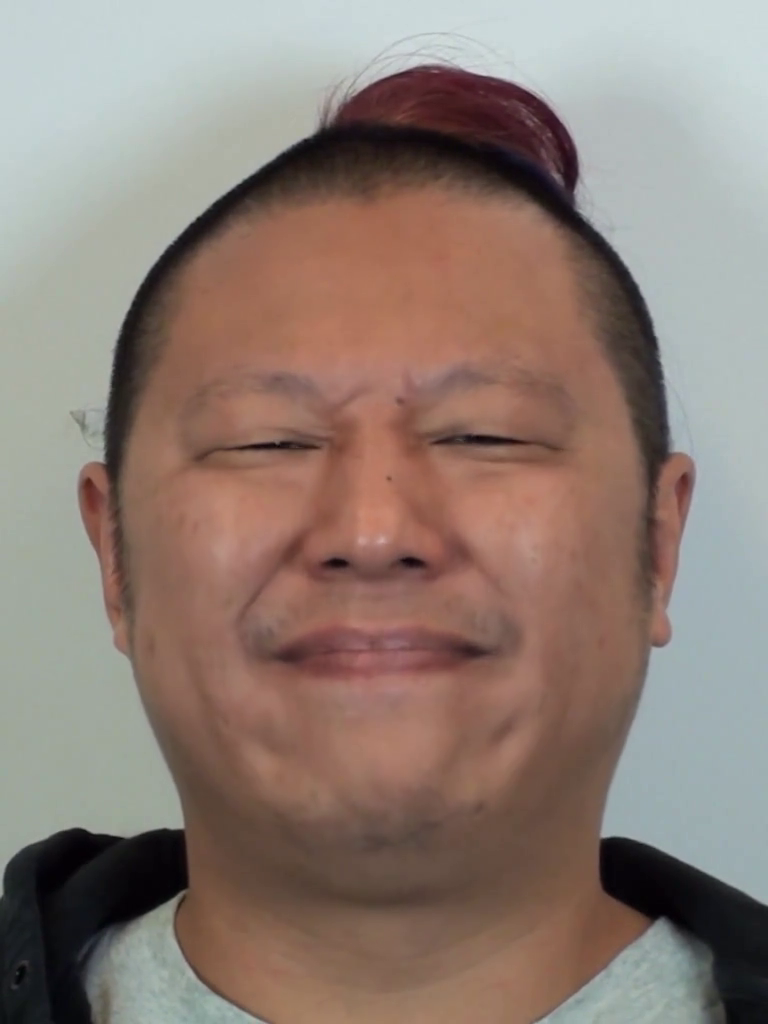
\includegraphics[width=0.32\columnwidth]{figures/haokyle_transfer/raw000681.png}
  %% \includegraphics[width=0.32\columnwidth]{figures/haokyle_transfer/static_000681.png}
  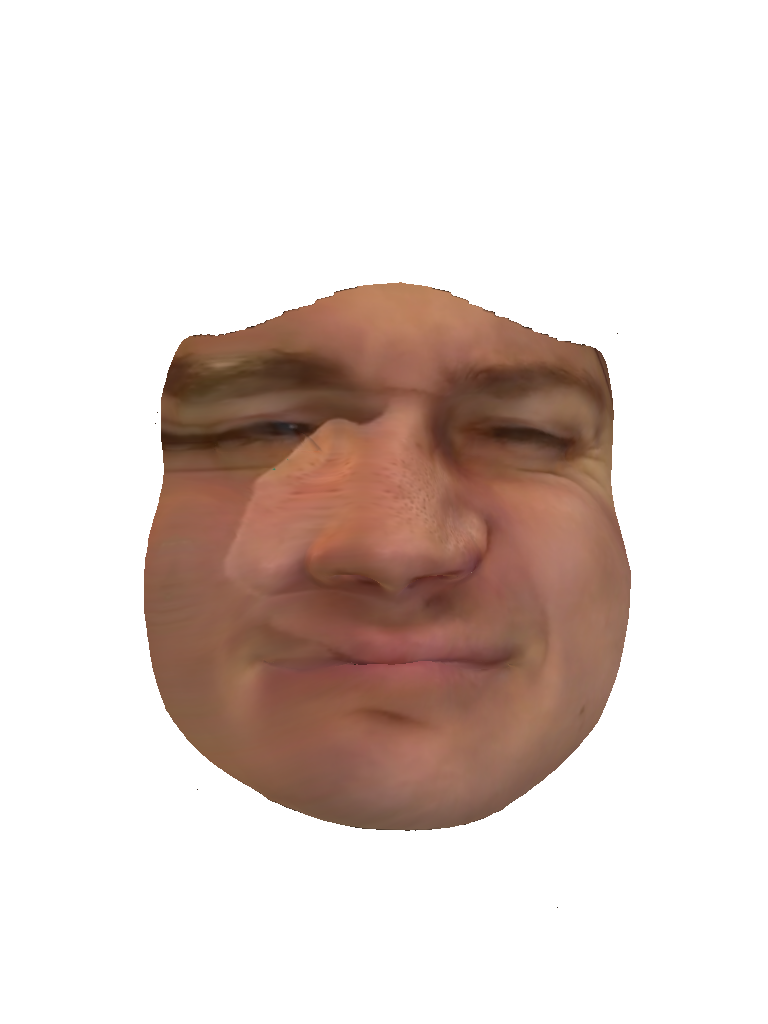
\includegraphics[width=0.32\columnwidth]{figures/haokyle_transfer/dynamic_000681.png}
\end{center}
   \caption{Failure cases induced by an extreme non-frontal target image. The top row displays the target image. The remaining rows display the source expression image (left) and the rendered image with the synthesized dynamic texture (right). While we can synthesize details for the visible region of the target image, the occluded regions contain artifacts that are visible when the image is rendered with these regions visible to the camera.}
   \vspace{-0.05in}
\label{fig:replaceres2}
\end{figure}

\begin{figure*}[h!]
\setlength\tabcolsep{1.5pt}
\centering
\begin{tabular}{cc}

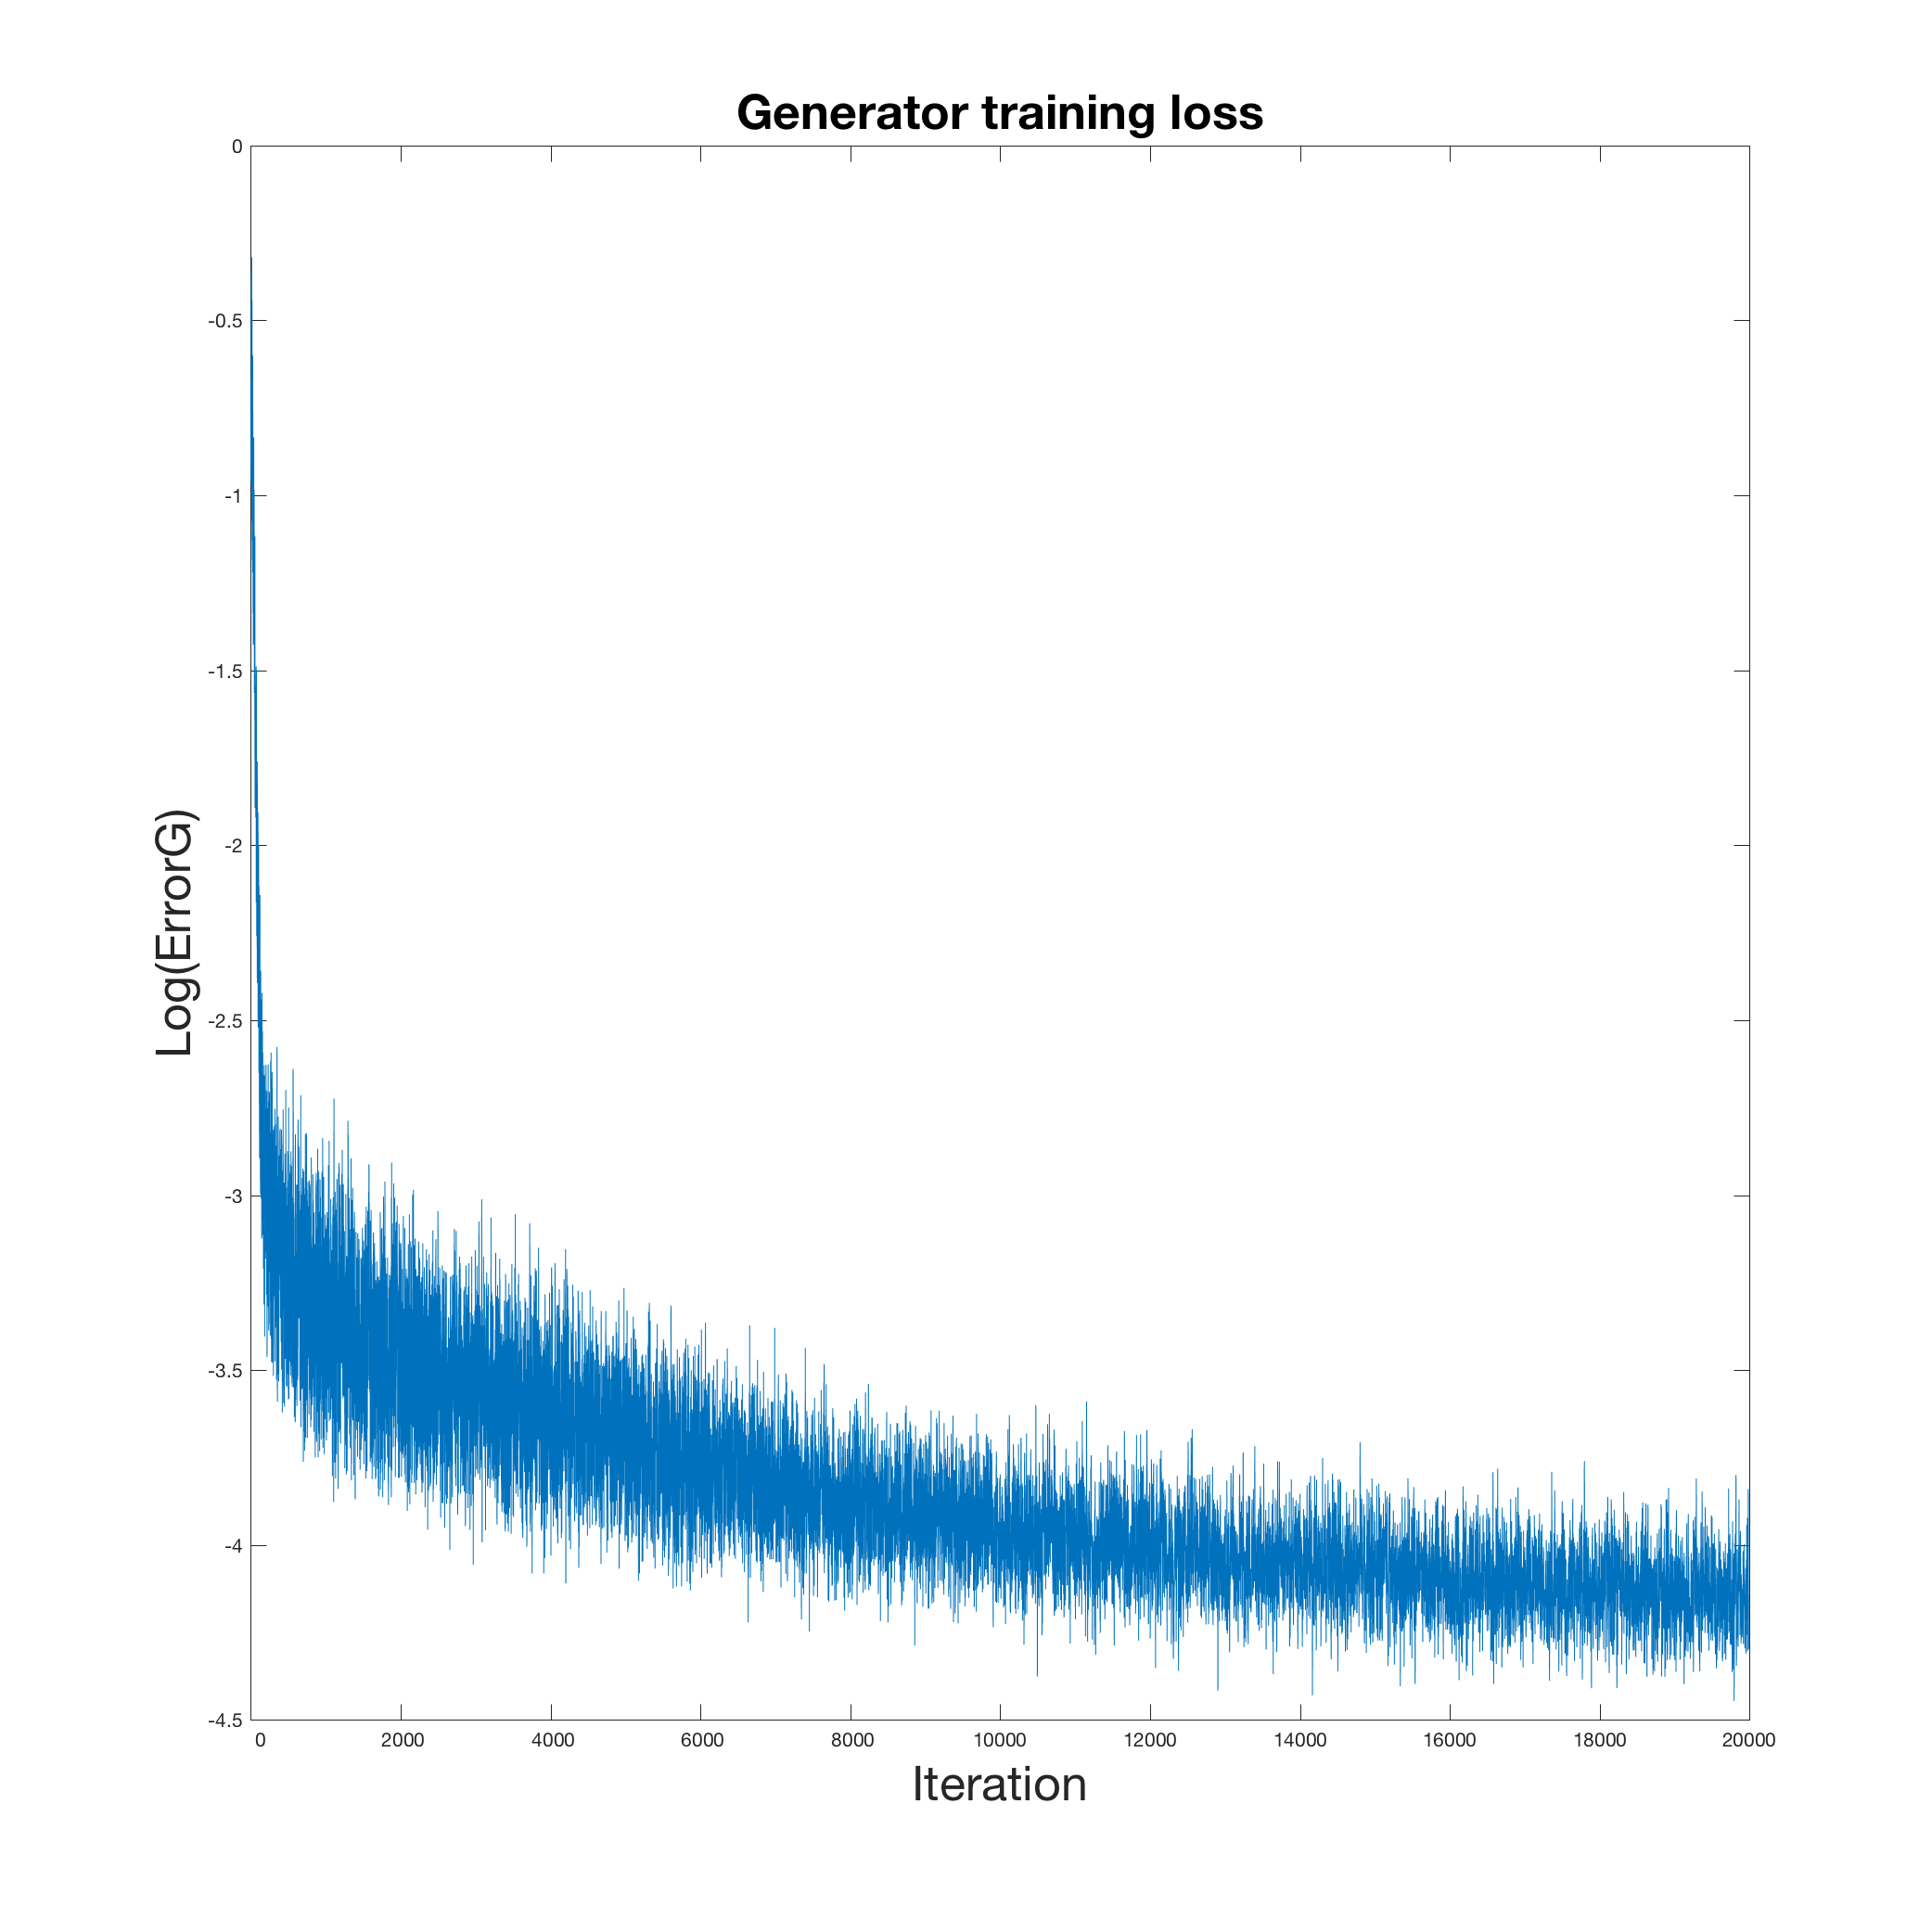
\includegraphics[width=.50\textwidth]{figures/loss/trainErrorG.png}&
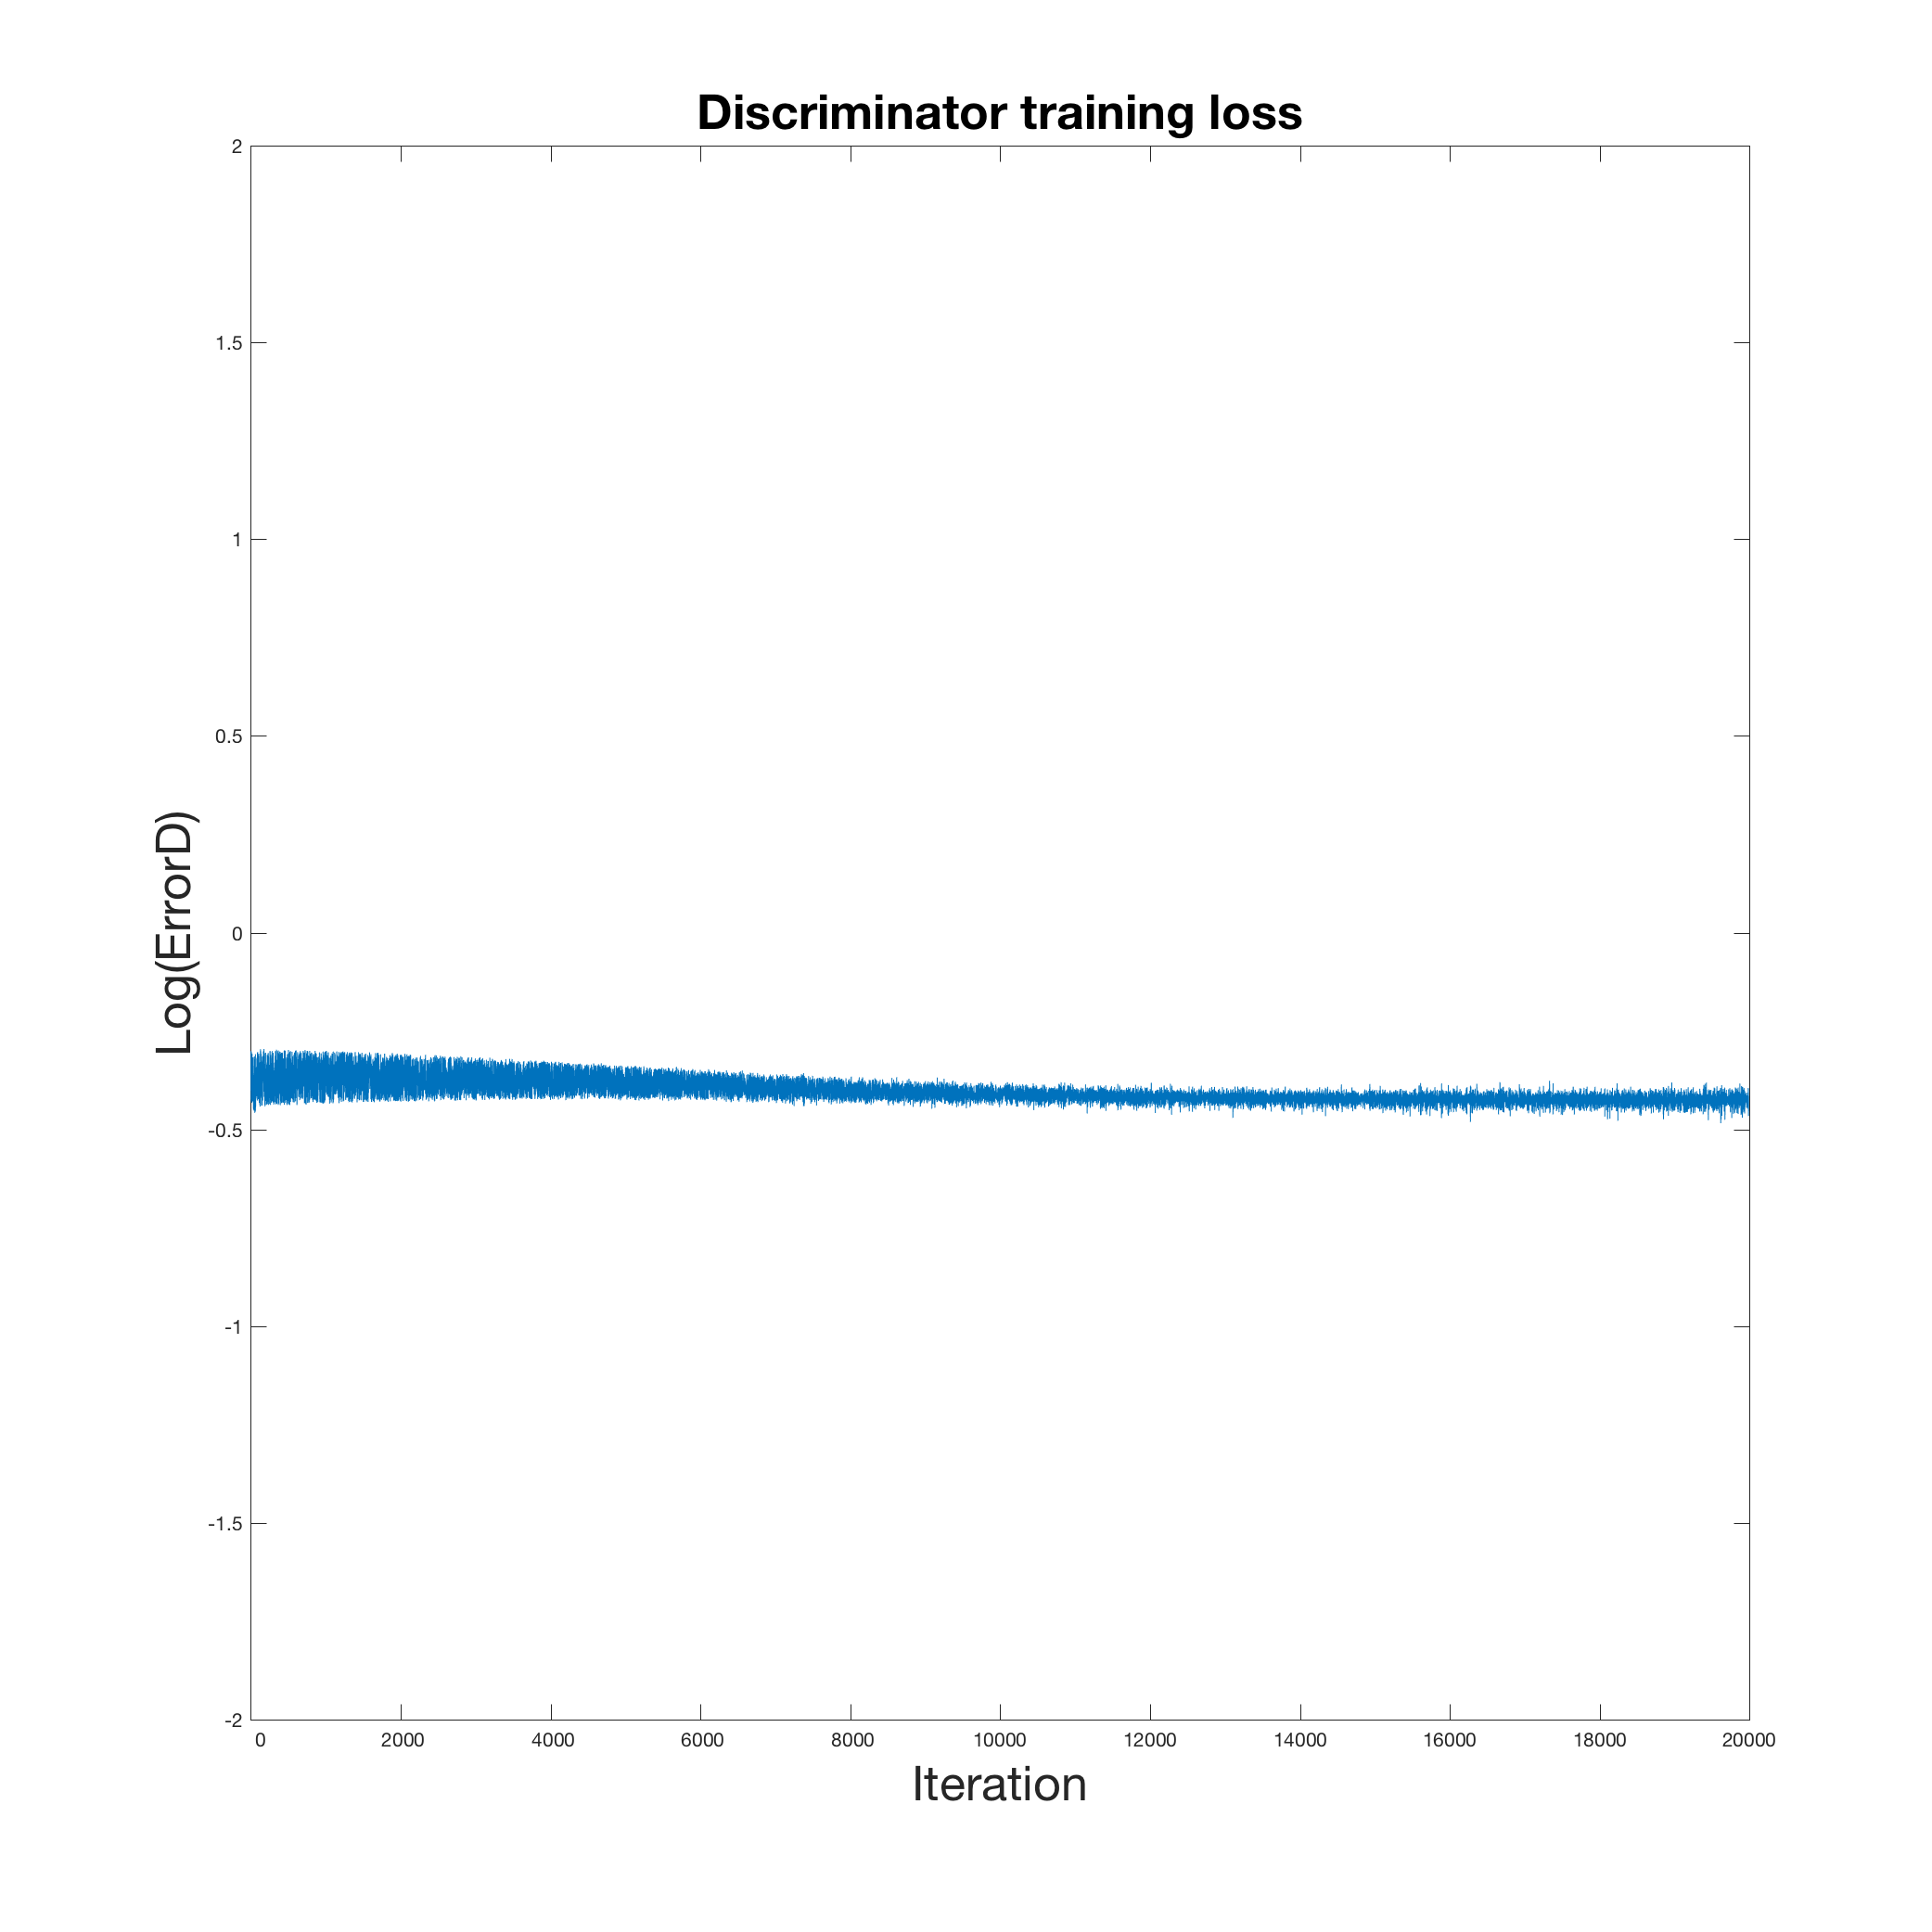
\includegraphics[width=.50\textwidth]{figures/loss/trainErrorD.png} \\
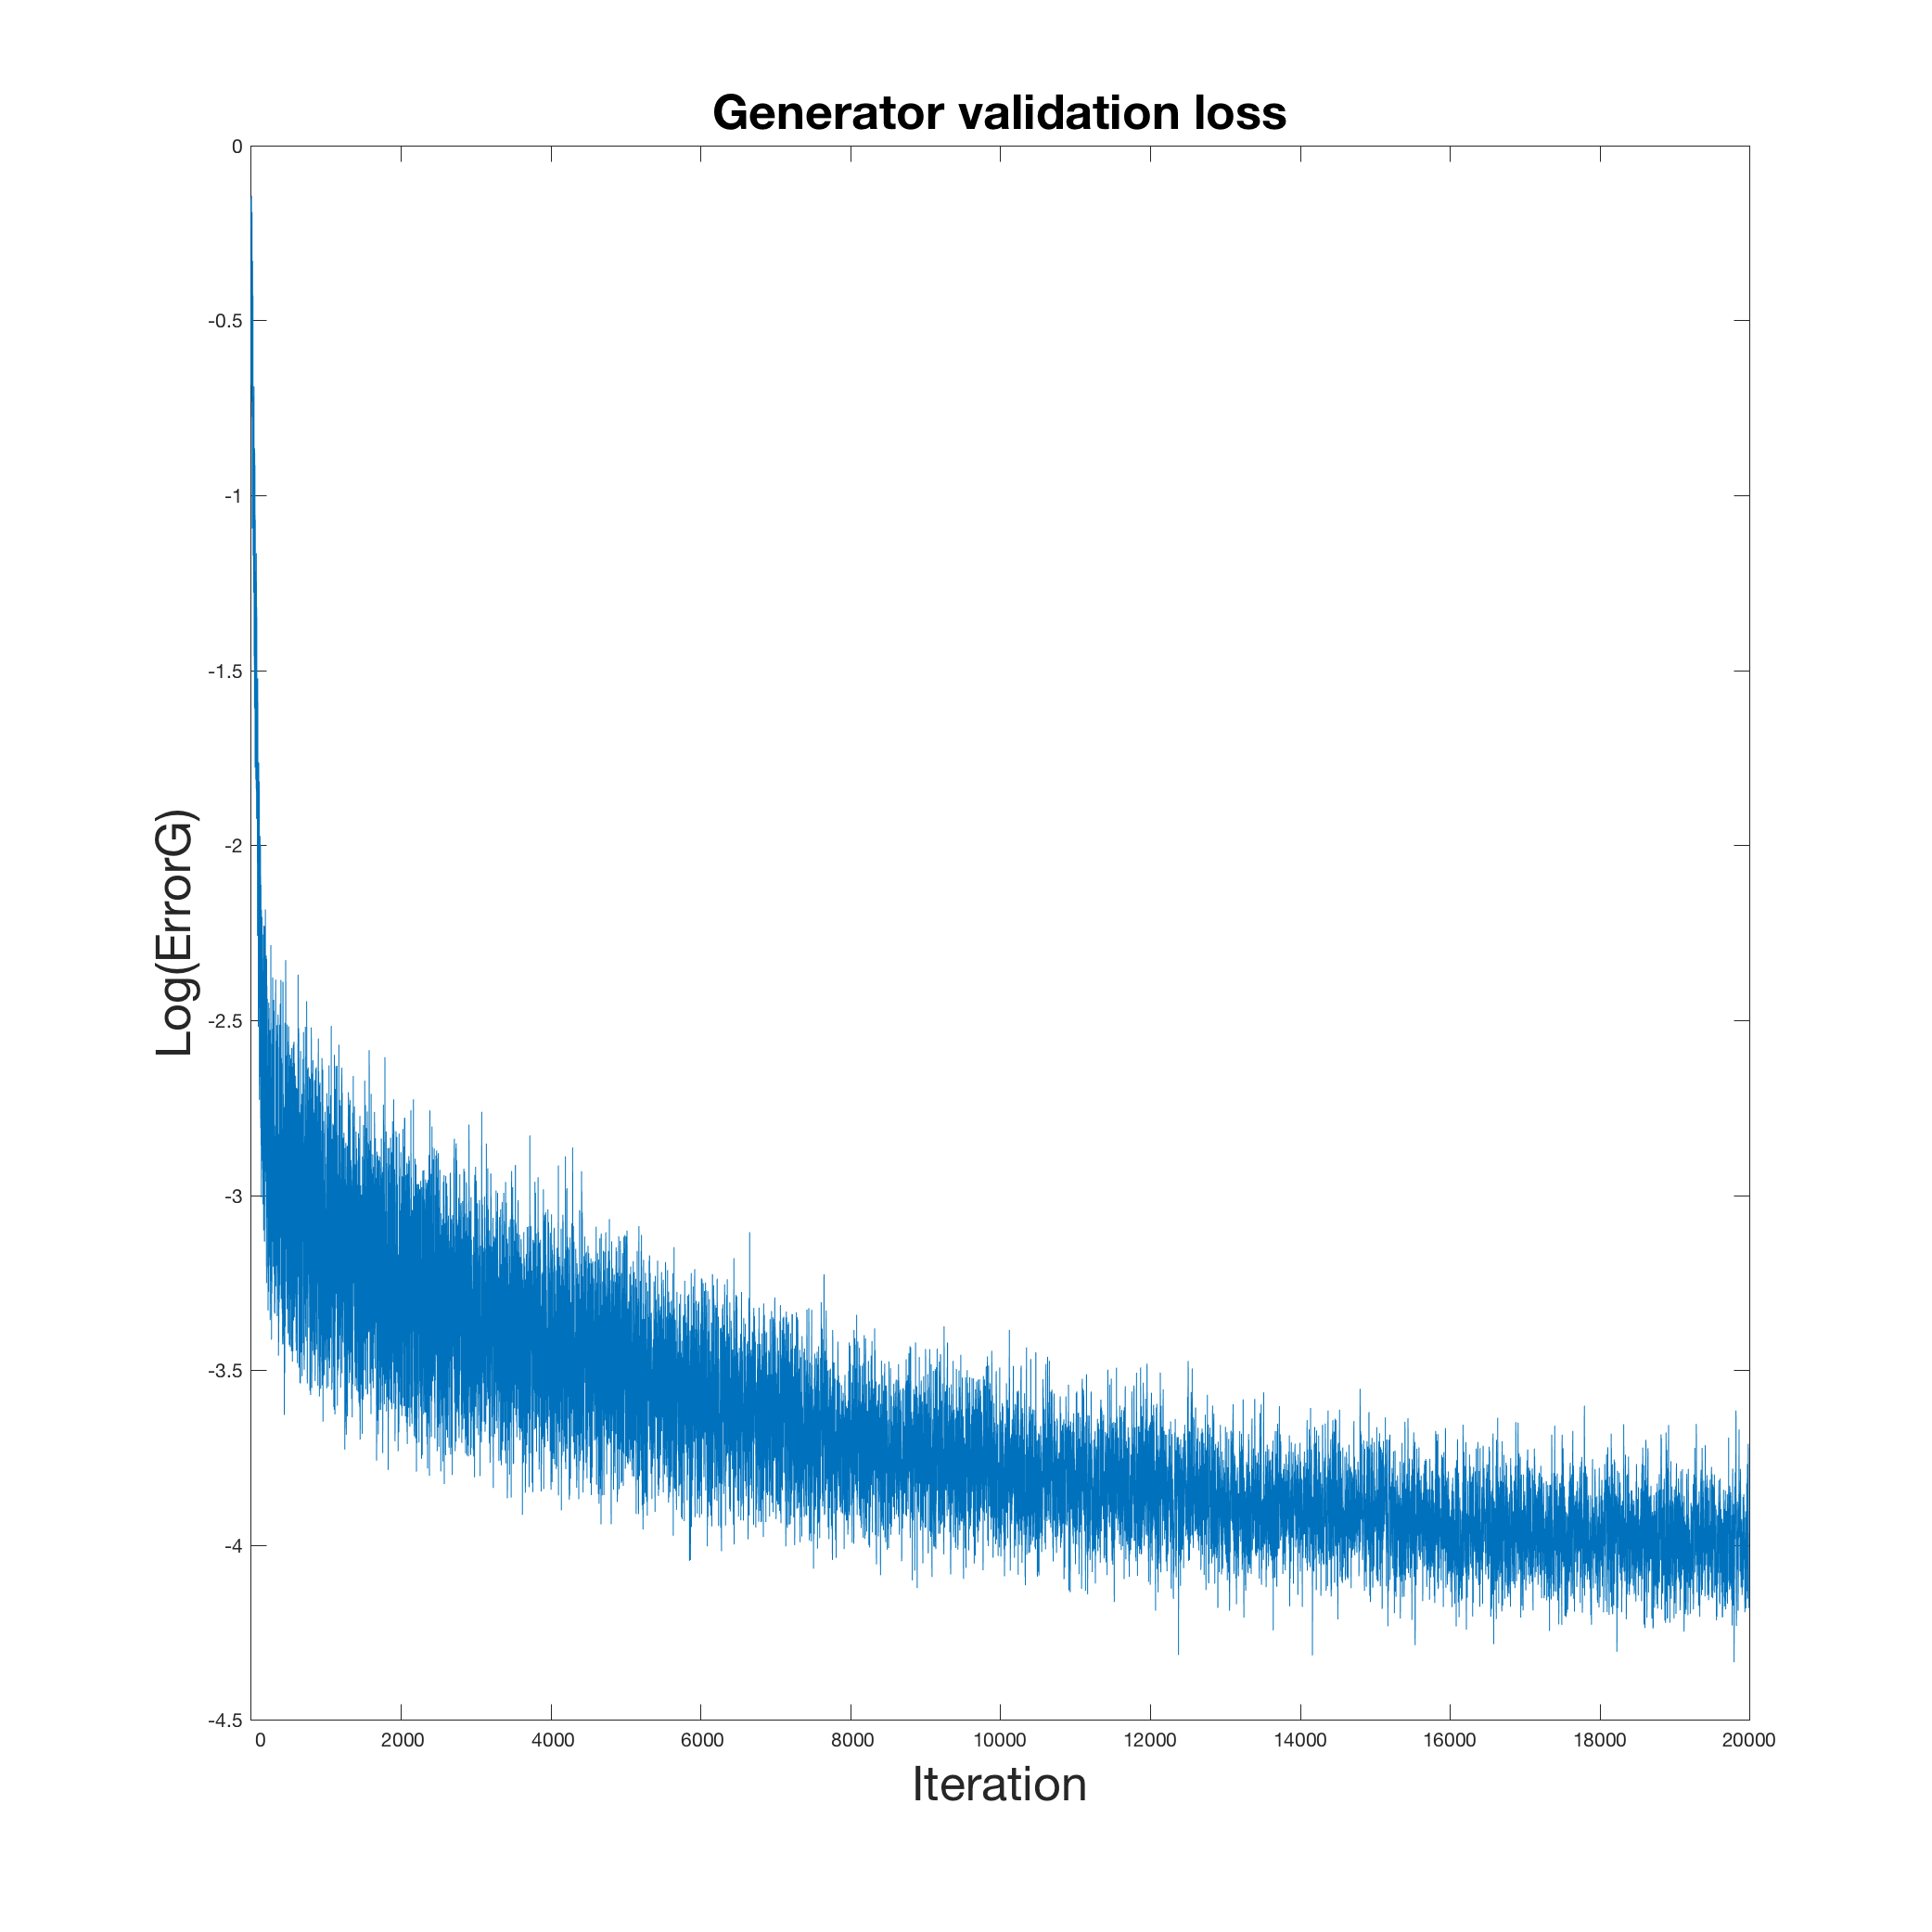
\includegraphics[width=.50\textwidth]{figures/loss/validErrorG.png}&
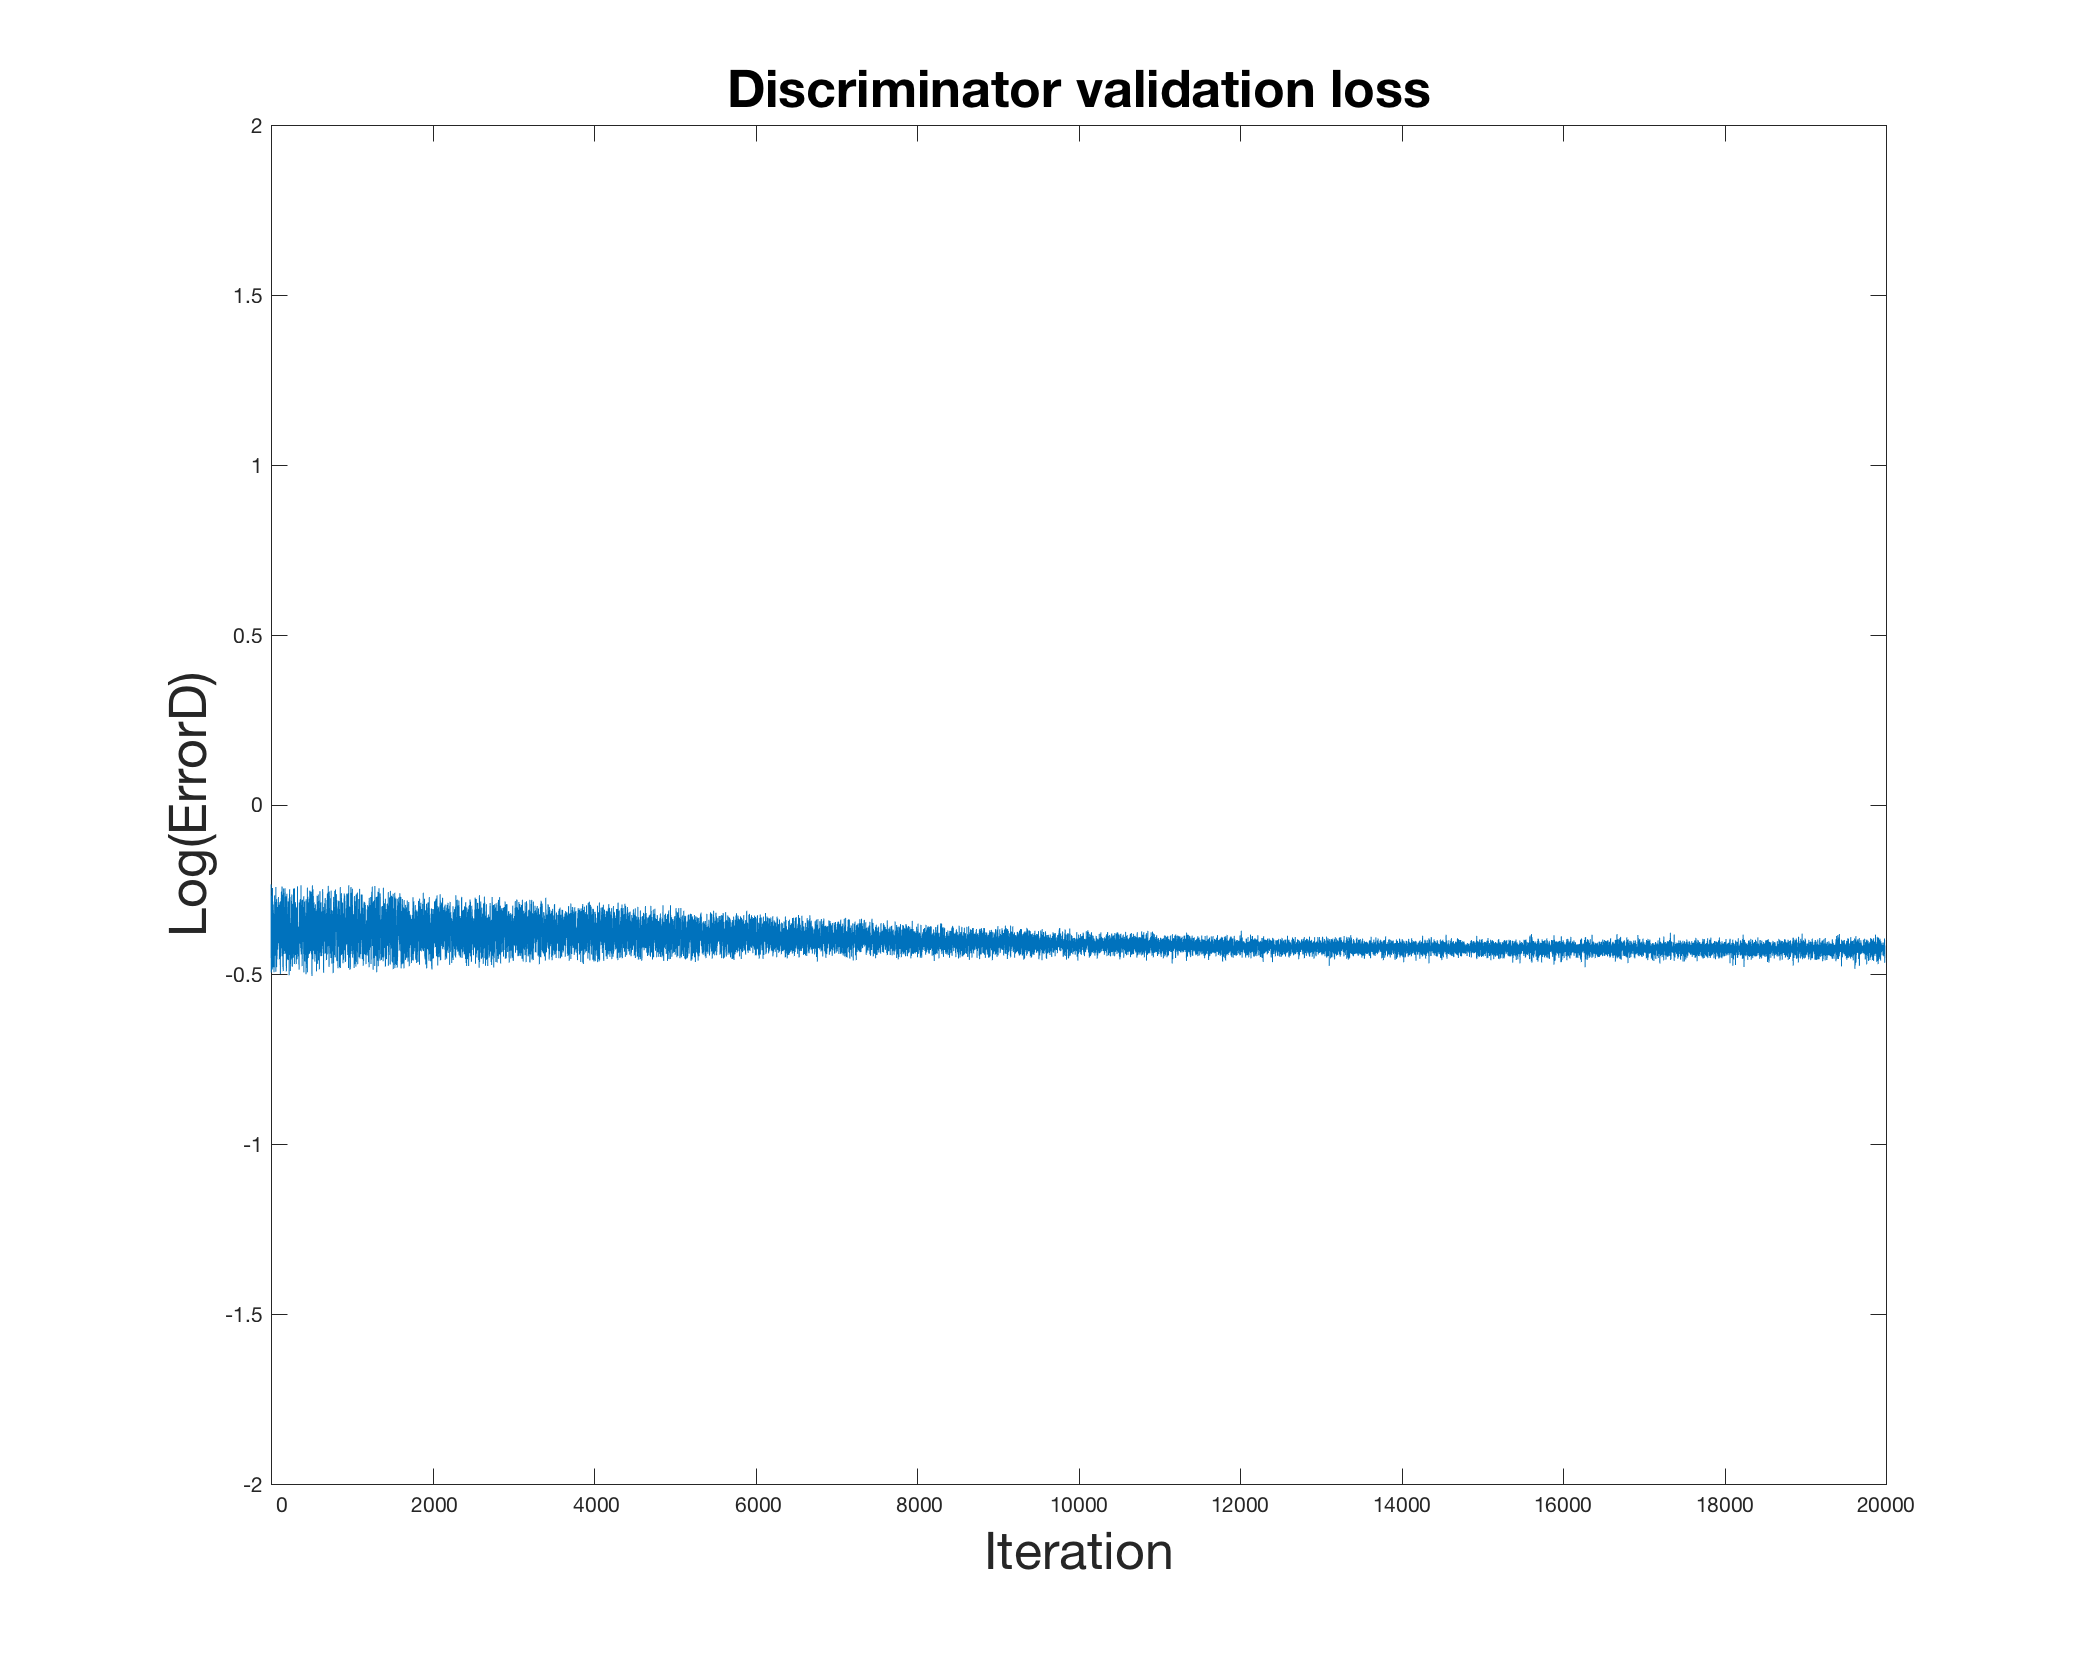
\includegraphics[width=.50\textwidth]{figures/loss/validErrorD.png} \\
Generator Error & Discriminator Error \\ 
\end{tabular}
\caption{Generative and discriminative training loss (top row) and validation loss (bottom row).}\label{fig:error}
\vspace{-0.05in}
\end{figure*}

\begin{figure*}[th]
\begin{center}
  \includegraphics[width=1.00\textwidth]{figures/supplementalresults.pdf} \\
\end{center}
  \caption{Additional retargeting and compositing results.}
  \vspace{-0.05in}
\label{fig:compositenew}
\end{figure*}

\end{document}
